\section{Modular Bin Strips\label{sec:innovation}}
  The previous section explained the operation of \gls{frnns} on \glspl{gpu} via the data structure \gls{usp}. In particular this research has concerned itself with optimisation at the stage of accessing bins. We have developed two independent optimisations that we refer to as \textit{Strips} and \textit{Modular}. These two optimisations can be combined to access the benefits of both techniques simultaneously.
  
  \note{Not too sure about consistent use of language here, neighbour or desired message etc. This also applies to the figure in the prior section.}
  
  In order to access all the messages within a given radius of the search position, we must check the contents of all the bins which may contain the desired messages. To achieve this we iterate the bins of the inclusive Moore neighbourhood of the search position's bin. In two dimensions this can be visualised as a 3x3 table containing 9 bins, and in three dimensions this can be visualised as cubes subdivided 3x3x3 into 27 bins. Naturally we iterate the Moore neighbourhood in a one bin at a time in a linear order, first following the X axis, then the Y and so forth, similar to how the labelling of the environment occurs. One example of this approach can be seen in NVIDIA's own particles example which implements uniform spatial partitioning.
  \note{CITE ME (NV Particles)}
  \subsection{Strips}
    The Strips optimisation targets redundant bin changes. Where a strip of bins within the Moore neighbourhood exists contiguously in memory, we clamp the strip's bins so that they are within the environment's bounds and  solely load the first bin's start index, and the last bin's end index from the partition boundary matrix.
    
    This optimisation essentially removes two bin changes from every central strip and one from every boundary strip. This occurs three times per neighbourhood in two dimensions and nine times in three dimensions. 
    
    Therefore the optimisation provides a near constant time speed up through removal of code, relevant to the problem dimensionality and number of simultaneous threads. Additionally the removal of the bin switches can reduce branch divergence, whereby threads within the same warp are operating on differently sized bins and hence would change bins at different times.
    
    \note{Also mention that is not easily applicable to space filling curves due to how they affect contiguous bins, but we tried them and found they were not a useful optimisation?}
    
    \note{Could include a code excerpt to show difference between bounds checking of default vs strips?}

  \subsection{Modular}
\begin{figure}[!t]
\centering
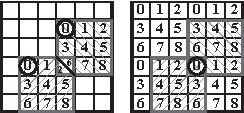
\includegraphics[width=\linewidth]{../resources/modular/modular.pdf}
\caption{\label{fig:modular}A visual representation of how the standard local indexing (left) and global indexing of the Modular optimisation (right) affect the iteration of two intersecting Moore neighbourhoods (marked grey). In the example shown, they both share the same initial bin under global indexing.}
\end{figure}
    The Modular optimisation targets scattered memory accesses. In the highly parallel \gls{gpu} execution, many neighbourhoods are being read simultaneously. Therefore it is almost certain that there will be intersecting Moore Neighbourhoods. Instead of iterating the Moore neighbourhood according to a local linear order, we calculate a recurring global index to define the order in which all Moore neighbourhoods are iterated. The global index can be produced by tightly packing linear indexed Moore neighbourhoods within the environment. Now when a Moore neighbourhood is positioned anywhere in the environment, it will contain one bin with each index value as shown in figure \ref{fig:modular}. Therefore it becomes possible to iterate the bins according to the order of their global indexes, such that the number of concurrent bins accessed is reduced significantly.
    
    The global index does not need to be precomputed, it can be computed at runtime with minimal additional instructions and storage.
    
    Instead of each thread independently tracking their current bin's relative position within the neighbourhood, the relative position is tracked at a block level and maintained by the first thread. When the search is initiated, the offset of the local Moore neighbourhood from the global Moore neighbourhood is calculated for each thread. When the relative and offset values are combined the result can be processed in a modular manner (bounded from $-1$ to $+1$) to provide the threads relative bin index. If not using block-level synchronisation, it becomes necessary to structure message iteration as a nested loop so that all threads within a block complete processing their bins before the block's relative bin is switched.
    %sm_message->state.relative = (*blockRelative)+sm_message->state.offset;
    %//For each axis, if new relative > 1, set -1
    %sm_message->state.relative.x = sm_message->state.relative.x>1 ? sm_message->state.relative.x - 3 : sm_message->state.relative.x;
    %...
    
    This optimisation reduces the maximum bins accessed to 1/9th of the environment in 2 dimensions and 1/27th in 3 dimensions. Thereby reducing unique memory loads, allowing more efficient utilisation of the limited memory and cache bandwidth.
    
    Although validation showed that the structure of the nested loop ensures synchronisation is maintained and all messages are accessed, we trialled including an explicit (and redundant) block synchronisation before bin changes. Testing however showed that this had a slight negative impact on the performance of the optimisation.
    %Additionally we trialled including a block synchronisation at each bin change, to ensure that the bin alignment remained consistent throughout iteration of the entire Moore neighbourhood without using a nested loop. Testing however showed that this had a slight negative impact on the performance of the optimisation.
    %\note{Add sample graph of sync vs !sync?}

  \subsection{Combining Strips \& Modular}
    The Strips optimisation as presented is only applicable to a single dimension, that which bins are contiguously stored in memory. On the other-hand the Modular optimisation is applicable to any dimensionality. Therefore it becomes possible to apply the Modular optimisation to the remaining dimensions of the Moore neighbourhood after the Strips optimisation has been applied.
    
    This loses the Modular optimisation from the first dimension in favour of the Strips optimisation, however the results in the next section show that this trade-off improves performance over that of either of the optimisations applied individually.
    
    %\note{Arguably we could maintain the modular optimisation by iterating messages within the strip from a modular offset, however this is not something we've tested. (It would require loading and storing more temporary iteration info).}